% !TeX root = status1.tex

\newcommand{\machineA}
{\begin{tikzpicture}[baseline=(current bounding box.center),shorten >=1pt,node distance=2.5cm,on grid,auto]
   \node[state,accepting] (q_0)   {$q_0$}; 
   \node[state,accepting] (q_1) [right=of q_0] {$q_1$}; 
    \path[->]
    (q_0) edge [bend left] node {$\neg a_0$} (q_1)
    (q_1) edge [bend left] node {$\bigvee_{i=0}^n a_i$} (q_0);
\end{tikzpicture}}

\newcommand{\machineAp}
{\begin{tabular}{c}
$\mathcal{P}(2^{\{a,b,c\}})$-SFA \\[5pt]
\begin{tikzpicture}[baseline=(current bounding box.center),shorten >=1pt,node distance=2.5cm,on grid,auto]
   \node[state,accepting] (q_0)   {$q_0$}; 
   \node[state,accepting] (q_1) [right=of q_0] {$q_1$}; 
    \path[->]
    (q_0) edge [bend left] node {$\neg a$} (q_1)
    (q_1) edge [bend left] node {$a \lor b \lor c$} (q_0);
\end{tikzpicture}
\end{tabular}}

\newcommand{\machineAoptp}
{\begin{tabular}{c}
$\big(\{a, \neg a \land (b \lor c), \neg (a \lor b \lor c\}\big)$-SFA \\[5pt]
\begin{tikzpicture}[baseline=(current bounding box.center),shorten >=1pt,node distance=2.5cm,on grid,auto]
   \node[state,accepting] (q_0)   {$q_0$}; 
   \node[state,accepting] (q_1) [right=of q_0] {$q_1$}; 
    \path[->]
    (q_0) edge [bend left] node {$\neg a$} (q_1)
    (q_1) edge [bend left] node {$a \lor b \lor c$} (q_0);
\end{tikzpicture}
\end{tabular}}

\newcommand{\machineB}
{\begin{tikzpicture}[baseline=(current bounding box.center),shorten >=1pt,node distance=2.5cm,on grid,auto]
   \node[state,accepting] (q_0)   {$q_0$};
   \node[state,accepting] (q_1) [right=of q_0] {$q_1$}; 
    \path[->]
      (q_0)
        edge [bend left,looseness=1.5,in=90,out=90]
          node {$\neg a_0 \land \bigvee_{i=1}^n a_i$}
        (q_1)
        edge [bend left]
          node {$\bigwedge_{i=0}^{n} \neg a_i$}
        (q_1)
      (q_1)
        edge [bend left]
          node {$a_0$}
        (q_0)
        edge [bend left,looseness=1.5,in=90,out=90]
          node {$\neg a_0 \land \bigvee_{i=1}^n a_i$}
        (q_0);
\end{tikzpicture}}

\newcommand{\machineBp}
{\begin{tabular}{c}
$\{a, \neg a \land (b \lor c), \neg (a \lor b \lor c\}$-NFA \\[5pt]
\begin{tikzpicture}[baseline=(current bounding box.center),shorten >=1pt,node distance=2.5cm,on grid,auto]
   \node[state,accepting] (q_0)   {$q_0$};
   \node[state,accepting] (q_1) [right=of q_0] {$q_1$}; 
    \path[->]
      (q_0)
        edge [bend left,looseness=1.5,in=90,out=90]
          node {$\neg a \land (b \lor c)$}
        (q_1)
        edge [bend left]
          node {$\neg (a \lor b \lor c)$}
        (q_1)
      (q_1)
        edge [bend left]
          node {$a$}
        (q_0)
        edge [bend left,looseness=1.5,in=90,out=90]
          node {$\neg a \land (b \lor c)$}
        (q_0);
\end{tikzpicture}
\end{tabular}}

\newcommand{\machineC}
{\begin{tabular}{c}
$\{000,001,010,011,100,101,110,111\}$-NFA \\[5pt]
\begin{tikzpicture}[baseline=(current bounding box.center),shorten >=1pt,node distance=2.5cm,on grid,auto]
   \node[state,accepting] (q_0)   {$q_0$};
   \node[state,accepting] (q_1) [right=of q_0] {$q_1$}; 
    \path[->]
      (q_0)
        edge [bend left,looseness=2.1,in=90,out=90] node {000} (q_1)
        edge [bend left,looseness=1.7,in=110,out=70] node {001} (q_1)
        edge [bend left,looseness=1.3,in=130,out=50] node {010} (q_1)
        edge [bend left,looseness=0.9,in=150,out=30] node {011} (q_1)
      (q_1)
        edge [bend left,looseness=3.5,in=70,out=110] node {111} (q_0)
        edge [bend left,looseness=3.0,in=80,out=100] node {110} (q_0)
        edge [bend left,looseness=2.5,in=90,out=90] node {101} (q_0)
        edge [bend left,looseness=2.0,in=100,out=80] node {100} (q_0)
        edge [bend left,looseness=1.5,in=110,out=70] node {011} (q_0)
        edge [bend left,looseness=1.0,in=120,out=60] node {010} (q_0)
        edge [bend left,looseness=0.5,in=130,out=50] node {001} (q_0);
\end{tikzpicture}
\end{tabular}}


\section{Transforming SFA to NFA}
\label{sect-transform}

As we noted in the preliminaries, because of the difference in language acceptance of SFAs and NFAs, language equivalence checking algorithms for NFAs are always sound, but necessarily not complete, when applied to SFAs. In this section we tackle the problem of reusing these algorithms for checking SFA language equivalence as well.

In subsection \ref{transform} we first present an obvious transformation that sends SFAs to NFAs, such that we can decide SFA language equivalence by checking NFA language equivalence of the transformed machines. Then in subsection \ref{optimize} we present a first optimization to this method using Veanes' minterms. Finally, we wrap up our argument in subsection \ref{wrapup}.

\subsection{SN transformation}
\label{transform}

\begin{definition}[SN Transformation]
\label{sn}
We define the transformation $\SN : \mathcal{S} \to \mathcal{N}$. Let $M = (Q, F, \Delta)$ be an SFA over the Boolean algebra $B$. Then $\SN(M)$ is the NFA $(Q, F, \Delta')$, over the alphabet $A_B$, where $(q,a,q') \in \Delta'$ iff $q \Trans{a} q'$.
\end{definition}

\begin{lem}
\label{sn-pres}
For any SFA $M$ we have the equality $\SL_M = \NL_{\SN(M)}$.
\end{lem}
\begin{proof}
Let $q \in Q_M = Q_{\SN(M)}$. By induction on the definition of $\SL_M(q)$ and $\NL_{\SN(M)}(q)$ we show that $\SL_M(q) \subseteq \NL_{\SN(M)}(q)$ and $\NL_{\SN(M)}(q) \subseteq \SL_M(q)$, respectively.
\begin{itemize}
\item Note that $\varepsilon \in \SL_M(q)$ iff $q \in F_M = F_{\SN(M)}$ iff $\varepsilon \in \NL_{\SN(M)}(q)$.
\item Let $aw \in \SL_M(q)$, say by $q \Trans{a}_M q'$ and $q \in \SL_M(q')$. By induction hypothesis $w \in \NL_{\SN(M)}(q')$, and by definition of $\SN(M)$ we have $q \trans{a}_{\SN(M)} q'$, and thus $aw \in \NL_{\SN(M)}(q)$.
\item Let $aw \in \NL_{\SN(M)}(q)$, say by $q \trans{a}_{\SN(M)} q'$ and $q \in \NL_{\SN(M)}(q')$. By induction hypothesis $w \in \SL_M(q')$ and by definition of $\SN(M)$ we have $q \Trans{a}_M q'$, and thus $aw \in \SL_M(q)$.
\end{itemize}
\end{proof}

The following figure depicts the transformation. An example is presented later on.

\begin{center}
\begin{tikzpicture}
  \matrix (m) [matrix of math nodes,row sep=2em,column sep=20em,minimum width=2em]
  {
     B\text{-SFA }M &
       A_B\text{-NFA }\SN(M) \\
  };
  \path[-stealth]
    (m-1-1)
      edge
        node [fill=white]
          {\begin{tabular}{c}
           $\SN$ transformation \\
           $\SL_M = \NL_{\SN(M)}$
          \end{tabular}}
          (m-1-2);
\end{tikzpicture}
\end{center}

\subsection{Alphabet optimization}
\label{optimize}

We have seen the SN transformation, which simply expands every arrow in the automaton to a set of arrows, one for each atom satisfying the formula on the original arrow. Running algorithms on the transformed automaton is, however, often very inefficient, because of the possibly exponential growth of the amount of arrows. We introduce an intermediate transformation $\opt : \mathcal{S} \to \mathcal{S}$, which we call \emph{alphabet optimization}, that reduces the size of the final SN transformed machine whilst preserving the language equivalence property. This optimization can be achieved in a similar fashion to how Veanes optimizes his minimalization algorithm, by using his previously introduced \emph{minterms}.

In a diagram, where we assume an SFA $M$ over a Boolean algebra $B$, and we have a particular, yet to be defined injection $e : \mathcal{P}(M(C)^*) \to \mathcal{P}({\mathfrak{A}_B}^*)$, and where $C = \{ \phi \mid \exists q,q',~q \trans{\phi} q' \} \subseteq B$, i.e.~the formulas occuring on arrows in $M$:

\begin{figure}[H]
\caption{The transformations}
\label{diagram}
\begin{center}
\begin{tikzpicture}
  \matrix (m) [matrix of math nodes,row sep=10em,column sep=20em,minimum width=2em]
  {
     B\text{-SFA }M &
       A_B\text{-NFA }\SN(M) \\
     (C)\text{-SFA }\opt(M) &
       M(C)
         \text{-NFA }\SN(\opt(M)) \\
  };
  \path[-stealth]
    (m-1-1)
      edge
        node [fill=white]
          {\begin{tabular}{c}
           alphabet optimization \\
           $\SL_M = e \circ \SL_{\opt(M)}$
          \end{tabular}}
          (m-2-1)
      edge
        node [fill=white]
          {\begin{tabular}{c}
           $\SN$ transformation \\
           $\SL_M = \NL_{\SN(M)}$
          \end{tabular}}
          (m-1-2)
    (m-1-2)
      edge [dotted,-]
        node [fill=white]
          {\begin{tabular}{c}
           $\NL_{\SN(M)} = e \circ \NL_{\SN(\opt(M))}$
          \end{tabular}}
          (m-2-2)
    (m-2-1)
      edge
        node [fill=white]
          {\begin{tabular}{c}
           $\SN$ transformation \\
           $\SL_{\opt(M)} = \NL_{\SN(\opt(M))}$
          \end{tabular}}
          (m-2-2);
\end{tikzpicture}
\end{center}
\end{figure}

\begin{definition}[Alphabet optimization]
Let $M = (Q,F,\Delta)$ be an SFA over a Boolean algebra $B$. Let $C = \{ \phi \mid \exists q,q',~q \trans{\phi} q' \} \subseteq B$. Consider the subalgebra $(C) \subseteq B$, which by definition contains $C$. Then simply define $\opt(M) = M$, but over the alphabet $(C)$.
\end{definition}

In the following we define a function $e : \mathcal{P}(M(C)^*) \to \mathcal{P}({\mathfrak{A}_B}^*)$ in the category of Boolean algebras using the Universal Mapping Property of the powerset: if we know the map on every singleton set, then it can be uniquely extended in such a way that unions are preserved.

\begin{definition}[Alphabet expansion]
Define the map $e_0$ by sending singletons $\{\varepsilon\} \mapsto \{\varepsilon\}$ and $\{mw\} \mapsto [m] \cdot e_0(\{w\})$, where ${\cdot}$ stands for language concatenation. Then we define $e : \mathcal{P}(M(C)^*) \to \mathcal{P}({\mathfrak{A}_B}^*)$ to be the unique extension of $e_0$ satisfying the powerset UMP.
\end{definition}

\begin{lem}
\label{opt-pres}
For any  SFA $M$ we have the equality $\SL_M = e \circ \SL_{\opt(M)}$.
\end{lem}
\begin{proof}
Let $q \in Q_M = Q_{\opt(M)}$. By induction on the definition of $\SL$ we prove that $\SL_M(q) \subseteq e(\SL_{\opt(M)}(q))$ resp.~$\SL_M(q) \supseteq e(\SL_{\opt(M)}(q))$.

Recall that any element $a \in B$ has exactly one minterm $m$ such that $a \le m$. Let us denote it $\overline{a} = m$. Overload this notation for words: $\overline{w} = \overline{a_1\dots a_n} = \overline{a_1} \dots \overline{a_n}$. Also note that, in general, by definition of $e$, we have $w \in X$ iff $\overline{w} \in e(X)$.

\begin{itemize}
\item First note that by definitions of $\SL$ and $e$, we have $\varepsilon \in \SL_M(q)$ iff $q \in F_M = F_{\opt(M)}$ iff $\varepsilon \in e(\SL_{\opt(M)}(q))$ iff $\varepsilon \in \SL_{\opt(M)}(q)$.
\item Proof of $\SL_M(q) \subseteq e(\SL_{\opt(M)}(q))$. Let $aw \in \SL_M(q)$. By definition of $\SL$ we have some $q' \in Q_M = Q_{\opt(M)}$ such that $q \TRANS{a}{M} q'$ and $w \in \SL_M(q')$. By the induction hypothesis we have $w \in e(\SL_{\opt(M)}(q'))$, and by definition of $e$ we know that $\overline{w} \in \SL_{\opt(M)}(q')$. Also, from $q \TRANS{a}{M} q'$ and $a \le \overline{a} \in A_{(C)}$ we can conclude that $q \TRANS{\overline{a}}{\opt(M)} q'$, and thus $\overline{aw} \in \SL_{\opt(M)}(q')$ by definition of $\SL$. Finally, by definition of $e$, we have $aw \in e(\SL_{\opt(M)}(q'))$.
%
\item Proof of $\SL_M(q) \supseteq e(\SL_{\opt(M)}(q))$. Let $aw \in e(\SL_{\opt(M)}(q))$. By definition of $e$ we must have $\overline{aw} \in \SL_{\opt(M)}(q')$. By definition of $\SL$ we have some $q'$ for which $q \TRANS{\overline{a}}{\opt(M)} q'$ and $\overline{w} \in \SL_{\opt(M)}(q')$. By the induction hypothesis we have $w \in \SL_M(q')$. Also, from $q \TRANS{\overline{a}}{\opt(M)} q'$ and $a \le \overline{a} \in A_{(C)}$ we can conclude that $q \TRANS{a}{M} q'$. Hence by definition of $\SL$ we have $aw \in \SL_M(q)$.
\end{itemize}
\end{proof}

\begin{lem}
\label{something-pres}
For any  SFA $M$ we have the equality $\NL_{\SN(M)} = e \circ \NL_{\SN(\opt(M))}$.
\end{lem}
\begin{proof}
This follows directly from Lemma \ref{opt-pres} and Lemma \ref{sn-pres}.
\end{proof}

\begin{example}
\label{ex37}

Consider the following SFA $M$ where $B$ is the free Boolean algebra over propositions $\{a_0, ..., a_n\}$:

\begin{center}
\machineA
\end{center}

Firstly, we compute the minterms of this automaton. These are given in the following tree:

\begin{equation*}
\begin{tikzpicture}
\Tree
[.{$\top$}
  {$a_0$}
  [.{$\neg a_0$}
    {$\neg a_0 \land \bigvee_{i=0}^n a_i$}
    {$\neg a_0 \land \neg \bigvee_{i=0}^n a_i$}
  ]
]
\end{tikzpicture}
\end{equation*}

Notice that:
\[\neg a_0 \land \bigvee_{i=0}^n a_i = \neg a_0 \land (a_0 \vee \bigvee_{i=1}^n a_i) = (\neg a_0 \land a_0) \vee (\neg a_0 \land \bigvee_{i=1}^n a_i) = \neg a_0 \land \bigvee_{i=1}^n a_i,\]
\[\neg a_0 \land \neg \bigvee_{i=0}^n a_i = \neg a_0 \land \bigwedge_{i=0}^{n} \neg a_i = \bigwedge_{i=0}^{n} \neg a_i.\] 
Hence, the minterms are $a_0$, $\neg a_0 \land \bigvee_{i=1}^n a_i$ and $\bigwedge_{i=0}^{n} \neg a_i$. We see the alphabet optimized and successively SN transformed automaton becomes:

\begin{center}
\machineB
\end{center}

Thus there are four transitions in the optimized automaton. However, if we used the normal automaton, the resulting automaton would be much larger. There are $2^{n-1}$ valuations in which $a_0$ holds, and there are $2^n - 1$ valuations in which $\bigvee_{i=0}^n a_i$ holds. Therefore, the resulting automaton of the SN Transformation would have $2^{n-1} + 2^{n} - 1$ transitions.

In the case that $P = \{a, b, c\}$ we have a situation as illustrated by Figure 2.

\begin{figure}
\caption{Example \ref{ex37} for the case of $P = \{a, b, c\}$}
\begin{center}
\begin{tikzpicture}
  \matrix (m) [matrix of math nodes,row sep=2em,column sep=8em,minimum width=2em]
  {
     \machineAp & \machineC \\
     \machineAoptp & \machineBp \\
  };
  \path[-stealth]
    (m-1-1)
      edge [draw=white,-]
        node [fill=white]
          {\rotatebox{-90}{$\stackrel{\text{AO}}{\scalebox{2}{$\longmapsto$}}$}}
          (m-2-1)
      edge [draw=white,-]
        node [fill=white]
          {$\stackrel{\text{SN}}{\scalebox{2}{$\longmapsto$}}$}
          (m-1-2)
    (m-1-2)
      edge [draw=white,-]
        node
          {}
          (m-2-2)
    (m-2-1)
      edge [draw=white,-]
        node [fill=white]
          {$\stackrel{\text{SN}}{\scalebox{2}{$\longmapsto$}}$}
          (m-2-2);
\end{tikzpicture}
\end{center}
\end{figure}

\end{example}


\subsection{Deciding SFA language equivalence}
\label{wrapup}

Regarding the transformations introduced, we finally state the main result justifying their existence. It proves that we can decide SFA language equivalence by checking NFA language equivalence of the SN transformed machines, and moreover do in an efficient manner, due to alphabet optimization.

\begin{thm}
Let $\mathcal{A}$ be any NFA language equivalence checking method, e.g.~$\mathcal{A} = \HKND$. For any SFA $M$ and states $q,q' \in Q_M$,
\begin{equation*}
\mathcal{A}_{\SN(\opt(M))}(q,q') \Iff
\mathcal{A}_{\SN(M)}(q,q') \Iff
\SL_M(q) = \SL_M(q').
\end{equation*}
\end{thm}

\begin{proof}
Because $\mathcal{A}$ is sound and complete for NFAs, we have $\NL_{\SN(M)}(q) = \NL_{\SN(M)}(q')$ iff $\mathcal{A}_{\SN(M)}(q,q')$. By Lemma \ref{sn-pres} we know that $\SL_M = \NL_{\SN(M)}$, and thus we have $\SL_M(q) = \SL_M(q')$ iff $\mathcal{A}_{\SN(M)}(q,q')$. This proves the second iff. For the first iff, this holds easily as well, noting that $\SL_M(q) = e \circ \SL_{\opt(M)}(q) = e \circ \SL_{\opt(M)}(q') = \SL_M(q')$ iff $\SL_{\opt(M)}(q) = \SL_{\opt(M)}(q')$.
\end{proof}

